\subsubsection*{Motoren}
\addcontentsline{toc}{subsubsection}{Motoren}


Nach ersten Berechnungen für die Motoren wurde ein passender Motor ausgewählt, bestellt und anschliessend getestet. Entscheidende Faktoren bei der Auswahl waren das Drehmoment und die Betriebsspannung.

\begin{figure}[H]
    \centering
    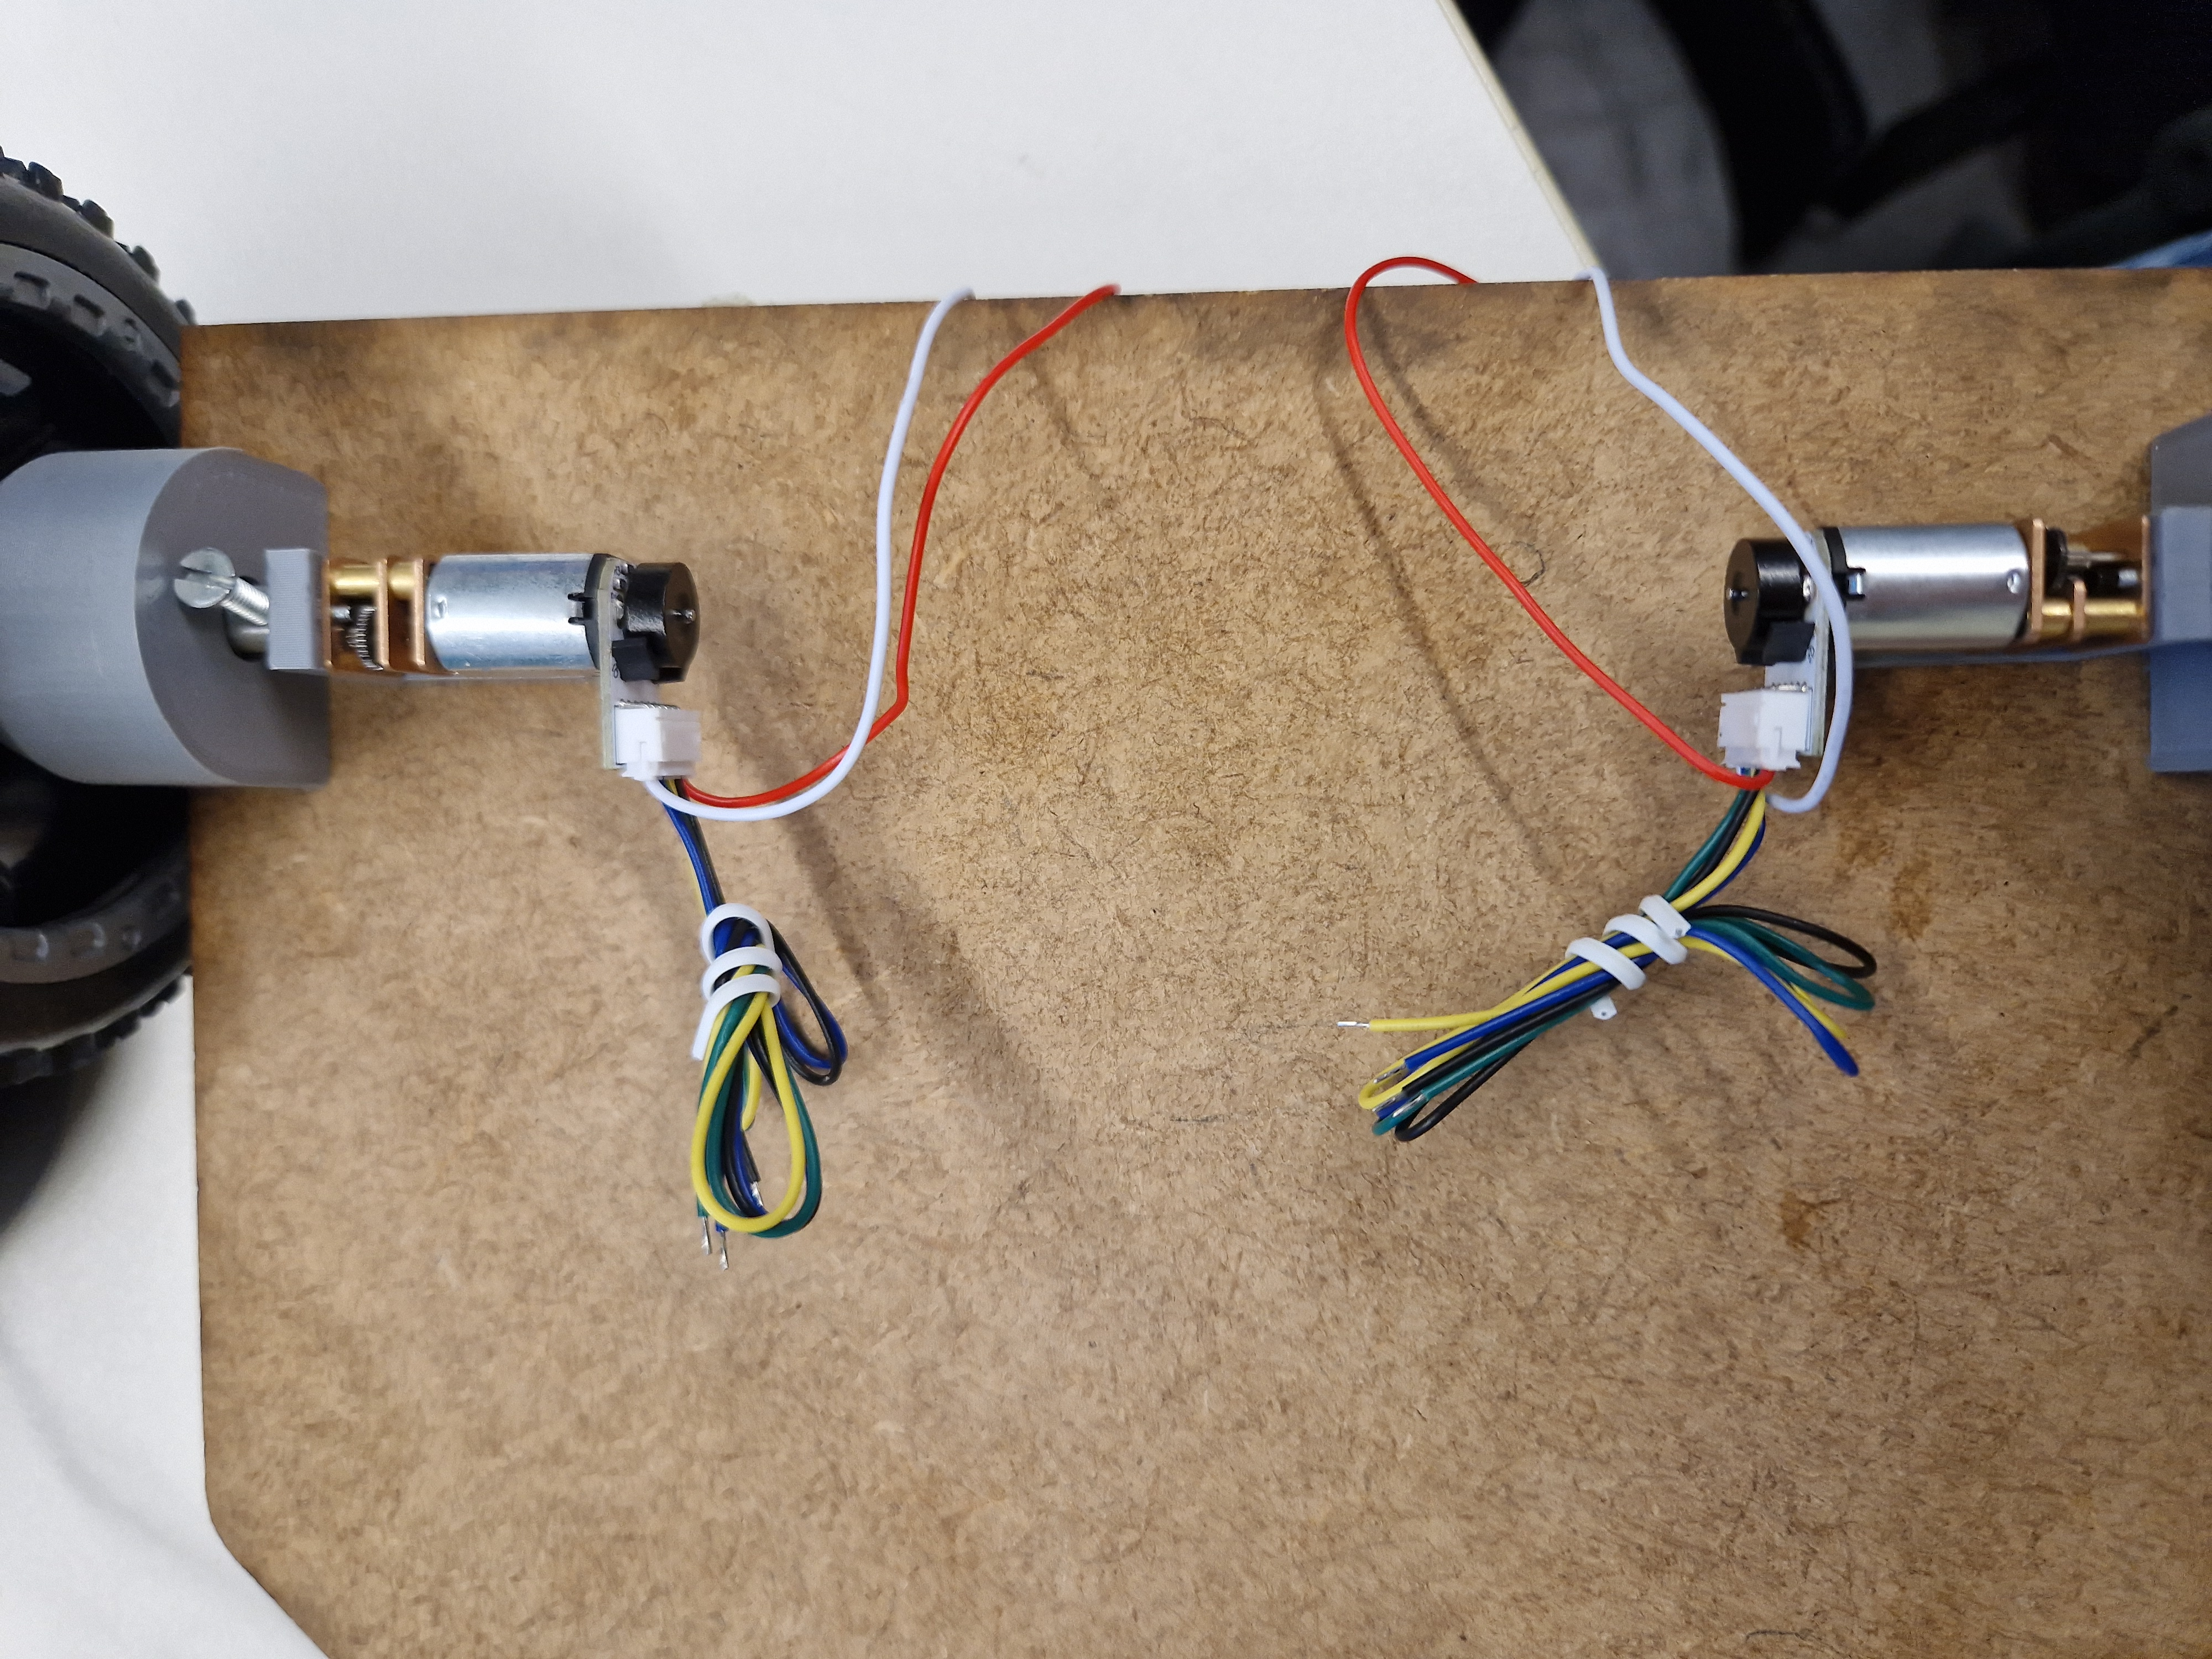
\includegraphics[width=0.8\linewidth]{img/Motorenaufbau.jpg}
    \caption{Motorenbefestigung Prototyp}
    \label{fig:Motorenaufbau}
\end{figure}

Der Test bestand darin, den Motor mit einer \acrfull{pwm} bei zwei unterschiedlichen Spannungen zu betreiben. Zunächst wurde der Motor mit einer Spannung von 5V getestet. Dabei wurde der Duty Cycle schrittweise erhöht, bis der Motor bei 58\% des Duty Cycles zu drehen begann. Nachdem der Motor angelaufen, konnte der Duty Cycle auf bis zu 44\% reduziert werden, bevor der Motor wieder stoppte.

In einer zweiten Testsequenz wurde die gleiche Vorgehensweise mit einer Spannung von 12V durchgeführt. Hier begann der Motor bei einem Duty Cycle von 33\% zu drehen. Beim schrittweisen Reduzieren der Einschaltzeit drehte der Motor bis zu einem Duty Cycle von 12\% weiter.

Da der Motor möglichst präzise gesteuert werden soll, ist eine feine Einstellung der Drehzahl erforderlich. Der Test zeigte jedoch, dass der Motor bei 5V nur verzögert anlief, was zu einer zu schnellen Drehbewegung führen könnte und die präzise Steuerung erschwert. Streuverluste sowie die Bauart des Motors erfordern einen höheren Anlaufstrom.

Um dennoch eine geringe Anfangsdrehzahl zu gewährleisten, wird der Motor initial mit 12V gestartet. Sobald der Motor angelaufen ist, wird die Spannung auf 5V reduziert, wodurch der Motor bei hohen Duty Cycle nicht Überlastet wird.

\begin{table}[H]
\centering
\begin{tabularx}{\textwidth}{|c|>{\centering\arraybackslash}X|>{\centering\arraybackslash}X|}
\hline
\textbf{Spannung} & \textbf{Einschaltzeit (Duty Cycle)} & \textbf{Ausschaltzeit (Duty Cycle)} \\ \hline
12V & 33\% & 12\% \\ \hline
5V  & 58\% & 44\% \\ \hline
\end{tabularx}
\caption{Vergleich der Duty-Cycle-Werte bei 12V und 5V}
\label{tab:dutycycle}
\end{table}

\subsubsection*{Tiny K22 Pinout} \label{Blockdiagramm: Schnittstellen zwischen den Komponenten}
\addcontentsline{toc}{subsubsection}{Tiny K22 Pinout}

Für die hardwarenahe Steuerung und Regelung wurde ein \acrshort{tinyk22} Version 1.4 ausgewählt, basierend auf der Methode des Morphologischen Kastens (Tab. \ref{table:mk-elektrotechnik}). Um die Software- und Hardwareauslegung des Projekts optimal zu gestalten, ist eine präzise Funktionszuweisung der einzelnen Pins erforderlich.

\begin{figure}[H]
    \centering
    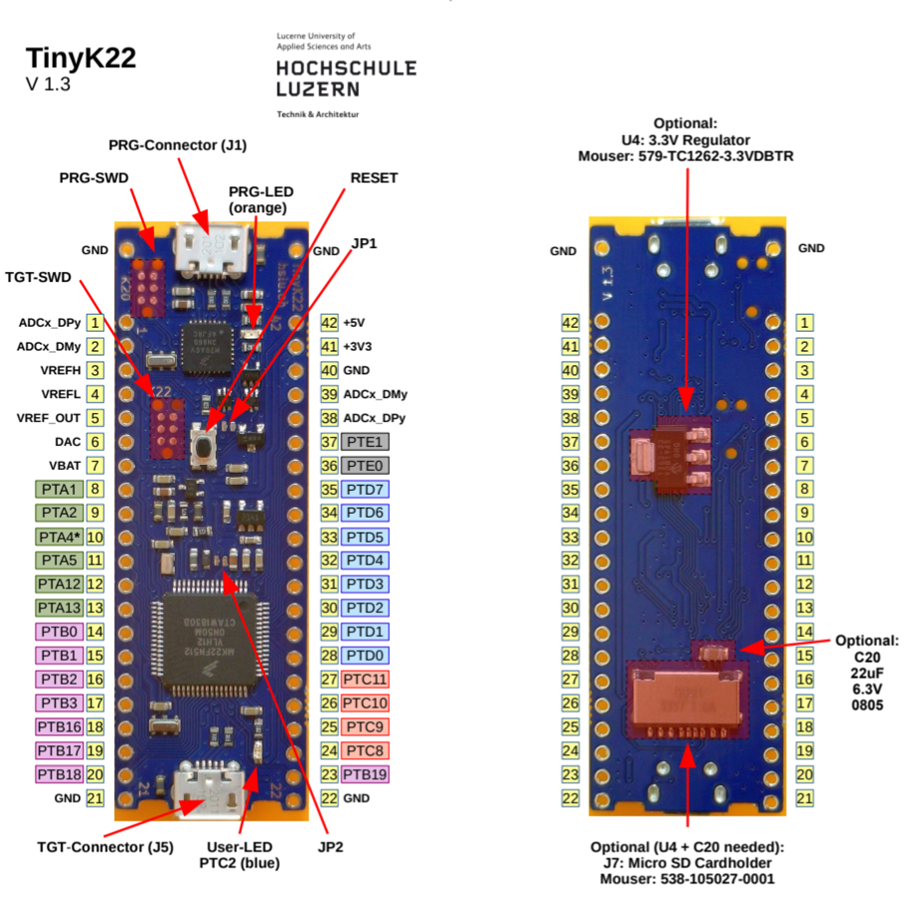
\includegraphics[width=0.8\linewidth]{img/Tiny_K22_PCB.png}
    \caption{Tiny K22. Quelle: \cite{tiny-K22-Pinout}}
    \label{fig:Tiny_K22_PCB}
\end{figure}


Das \acrshort{tinyk22} \acrshort{pcb} bietet insgesamt 28 Pins (Abb. \ref{fig:Tiny_K22_PCB}). Diese Pins können flexibel als \acrfull{ftm}, \acrfull{adc}, \acrfull{iic}, \acrfull{spi}, \acrshort{uart}, Input- oder Output-Pins konfiguriert werden.

Im Rahmen des Projekts wurden 25 Pins verwendet (Abb. \ref{fig:Tiny_K22_Pinout_definition}). Die zeitkritischen Funktionen werden direkt auf dem \acrshort{tinyk22} verarbeitet. Dabei werden folgende Zuweisungen vorgenommen:

\begin{figure}[H]
    \centering
    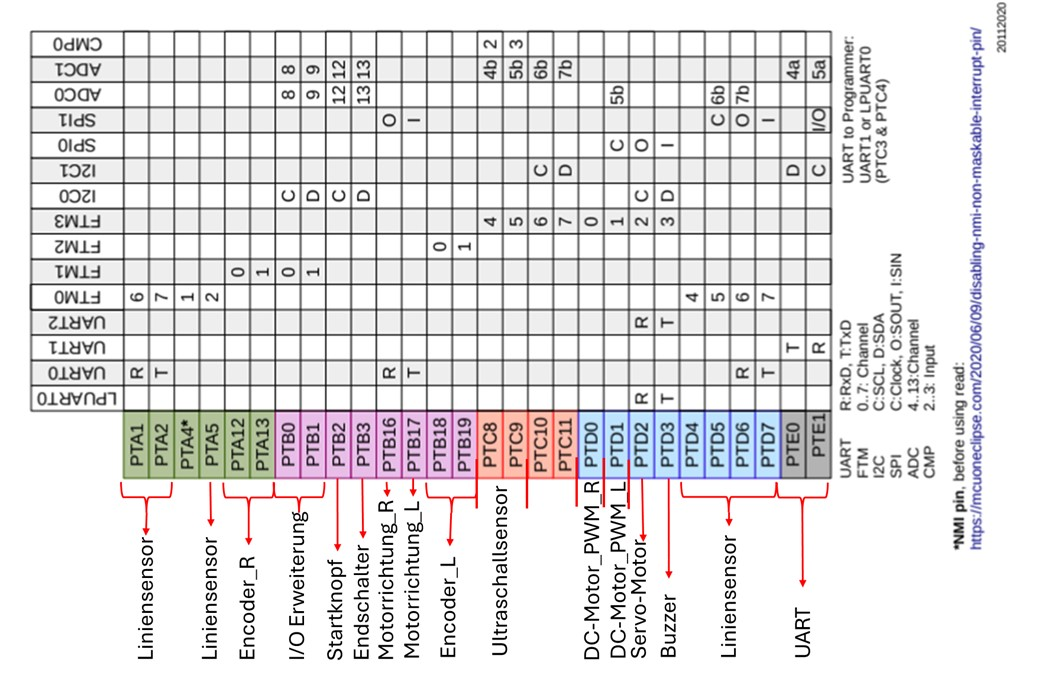
\includegraphics[width=0.8\linewidth, angle=-90]{img/Tiny_K22_Pinout_definition.jpg}
    \caption{Pinout Tiny K22. Quelle: \cite{tiny-K22-Pinout}}
    \label{fig:Tiny_K22_Pinout_definition}
\end{figure}

Encoder-Auswertung: Der Mikrocontroller nutzt die integrierte Quadratur-Encoder-Auswertung auf Timer 1 und Timer 2.
 \newline Linienerfassung: Diese Funktion belegt den gesamten Timer 0.
 \newline Motorsteuerung, Ultraschallsensor, Buzzer und Servomotor: Diese teilen sich Timer 3, da keine weiteren Timer zur Verfügung stehen. Dies führt dazu, dass die Motoren im hörbaren Frequenzbereich betrieben werden. Dieser Umstand ist jedoch akzeptabel, da keine Vorgaben zur maximalen Lautstärke existieren.
Zusätzlich wird ein \acrshort{iic}-Bus für zeitunkritische Funktionen verwendet. Zu diesen gehören die Ziellampe und die Zielauswahlschalter.

Durch diese Zuweisung wird sichergestellt, dass die zeitkritischen Aufgaben effizient verarbeitet werden, während gleichzeitig Flexibilität für zusätzliche Funktionen über den \acrshort{iic}-Bus gewährleistet bleibt.

\subsubsection*{Software Steuerung}
\addcontentsline{toc}{subsubsection}{Software Steuerung}


Das Programm welches man auf das \acrshort{tinyk22} laden wird, wird in C geschrieben. Mit der Entwicklungsumgebung MCUXpressoIDE kann der Code geschrieben und kompiliert werden. Debuggen kann man das Programm ebenfalls, da auf dem Tiny K22 ein Debugger beinhaltet ist. Es können vom Modul ``Mikrocontroller Fundamentals'' bestehende Libraries verwendet werden. Einige Anpassungen wie zum Beispiel die \acrshort{uart} wurden bereits vorgenommen.

\subsubsection*{Liniensensor}
\addcontentsline{toc}{subsubsection}{Liniensensor}


Der Liniensensor wird als Array verwendet, das heisst es werden Sensoren nebeneinander auf dem \acrshort{pcb} angeordnet. Es sind 7 Pins auf dem \acrshort{tinyk22} reserviert (Abb. \ref{fig:Tiny_K22_Pinout_definition}). Die 7 Pins werden die einzelnen Sensoren auslesen und die Werte verarbeiten. Mithilfe von Kondensatoren werden die Entladezeiten für die Auswertung genutzt (Abb. \ref{fig:Liniensensor_Schaltung}). Mit der Timerfunktion \verb|Input Capture| kann die bei Entladung fallende Flanke detektiert werden. \verb|Input Capture| gibt die Zeit zurück von dem Zeitpunkt bei dem der Kondensator sich anfängt zu entladen bis die Spannung 0V ist.

\begin{figure}[H]
    \centering
    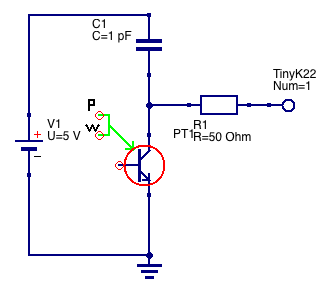
\includegraphics[width=0.8\linewidth]{img/Liniensensor_Schaltung.png}
    \caption{Schaltungsprinzip Liniensensor}
    \label{fig:Liniensensor_Schaltung}
\end{figure}

\subsubsection*{Ultraschall}
\addcontentsline{toc}{subsubsection}{Ultraschall}


Damit man die Hindernisse detektieren kann wird ein Ultraschallsensor verwendet. In dem man die Laufzeit der zurück empfangenen Ultraschallwellen auswertet, wird der Abstand zwischen Hindernis und Fahrzeug berechnet. Der Ultraschallsensor wird sich im vorderen Teil des Fahrzeugs befinden, damit eine freie Sicht gewährleistet ist und keine Störungen durch das Fahrzeug selbst auftreten.

\subsubsection*{Akku}
\addcontentsline{toc}{subsubsection}{Akku}


Um das ganze System mit Spannung zu versorgen wird ein 14.8V Akku verwendet. Dieser liefert in einer Stunde 3000mA. Bei einer geschätzten maximalen Leistung von 30W und einer Spannung von 12V reicht diese Kapazität für ca. 1.2 Stunden. 

\subsubsection*{PCB Design}
\addcontentsline{toc}{subsubsection}{PCB Design}


Das \acrshort{pcb} wird aus mehreren Teilen bestehen. Das Mainboard wird zentral eingebaut da es der Knotenpunkt ist und der grösste \acrshort{pcb} Komponent ist. Ebenfalls wird eine seperate Platine für die Spannungsversorgun benötigt, welches sich ebenfall zentral befinden wird. Der Ultraschall- und Liniensensor befinden sich im vorderen Teil des Roboters und werden über eine Kabelverbindung mit dem Mainboard erschlossen. Aufgrund der Wiederverwendung wird man die einzelnen Komponenten wie auch das \acrshort{tinyk22} steckbar verbinden. Das die Produktionskosten und der Abfall auf ein minimum reduziert werden wird man die verschiedenen \acrshort{pcb} als Einzelstück produzieren lassen und die Stücke mit brechen von einander lösen.

\subsubsection*{Servomotor}
\addcontentsline{toc}{subsubsection}{Servomotor}


Der Servomotor wurde direkt am Greifer Prototyp getestet. In der folgenden Tabelle \ref{tab:testpunkte Servomotor} sind die Messergebnisse eingetragen, welche positiv ausgefallen sind. Man hat den Servomotor bei zwei unterschiedlichen Frequenzen, mit der Betriebsspannung von 5V und ob das Hindernis auf die geforderten 7.5mm angehoben werden kann, getestet. Das \acrshort{pwm} Signal hat man mit einem Tektronix AFG1022 generiert, bei dem man mit dem Drehregler den Duty Cycle verstellen konnte.

\textbf{Messungen und Beobachtungen}

\begin{table}[H]
\centering
\small
\begin{tabularx}{\textwidth}{|c|X|X|X|l|}
        \hline
        \textbf{Index} & \textbf{Kurzbeschreibung} & \textbf{Kriterium zur Erfüllung} & \textbf{Messergebnisse} & \textbf{Bemerkungen} \\
        \hline
        1 & PWM mit 10kHz & Motor soll drehen & Der Motor dreht nicht & Test nicht erfüllt \\ \hline
        2 & PWM mit 400Hz & Motor soll drehen & bei 15\% Duty Cycle dreht Servomotor 180 Grad & Test erfüllt \\ \hline
        3 & Betriebsspannung mit 5V & Betrieb damit \acrshort{pwm} funktioniert  & PWM funktioniert & Test erfüllt\\ \hline
        4 & Motor drehen bis Hindernis angehoben & Hindernis wird angehoben & Greifer hebt Hindernis 7.5mm hoch, bei 32\% Duty Cylce & Test erfüllt \\ \hline
\end{tabularx}
    \caption{Testergebnisse des Servomotors am Greifer.}
\label{tab:testpunkte Servomotor}
\end{table}

\newpage

Der Startpunkt des Tests wurd bei einem Duty Cycle von 86\% festgelegt. Wie in der Abbildung \ref{fig: Greiferposition offen: Duty Cycle 86} ersichtlich wird, war das die Position, bei welcher der Greifer offen ist.

\begin{figure}[H]
    \centering
    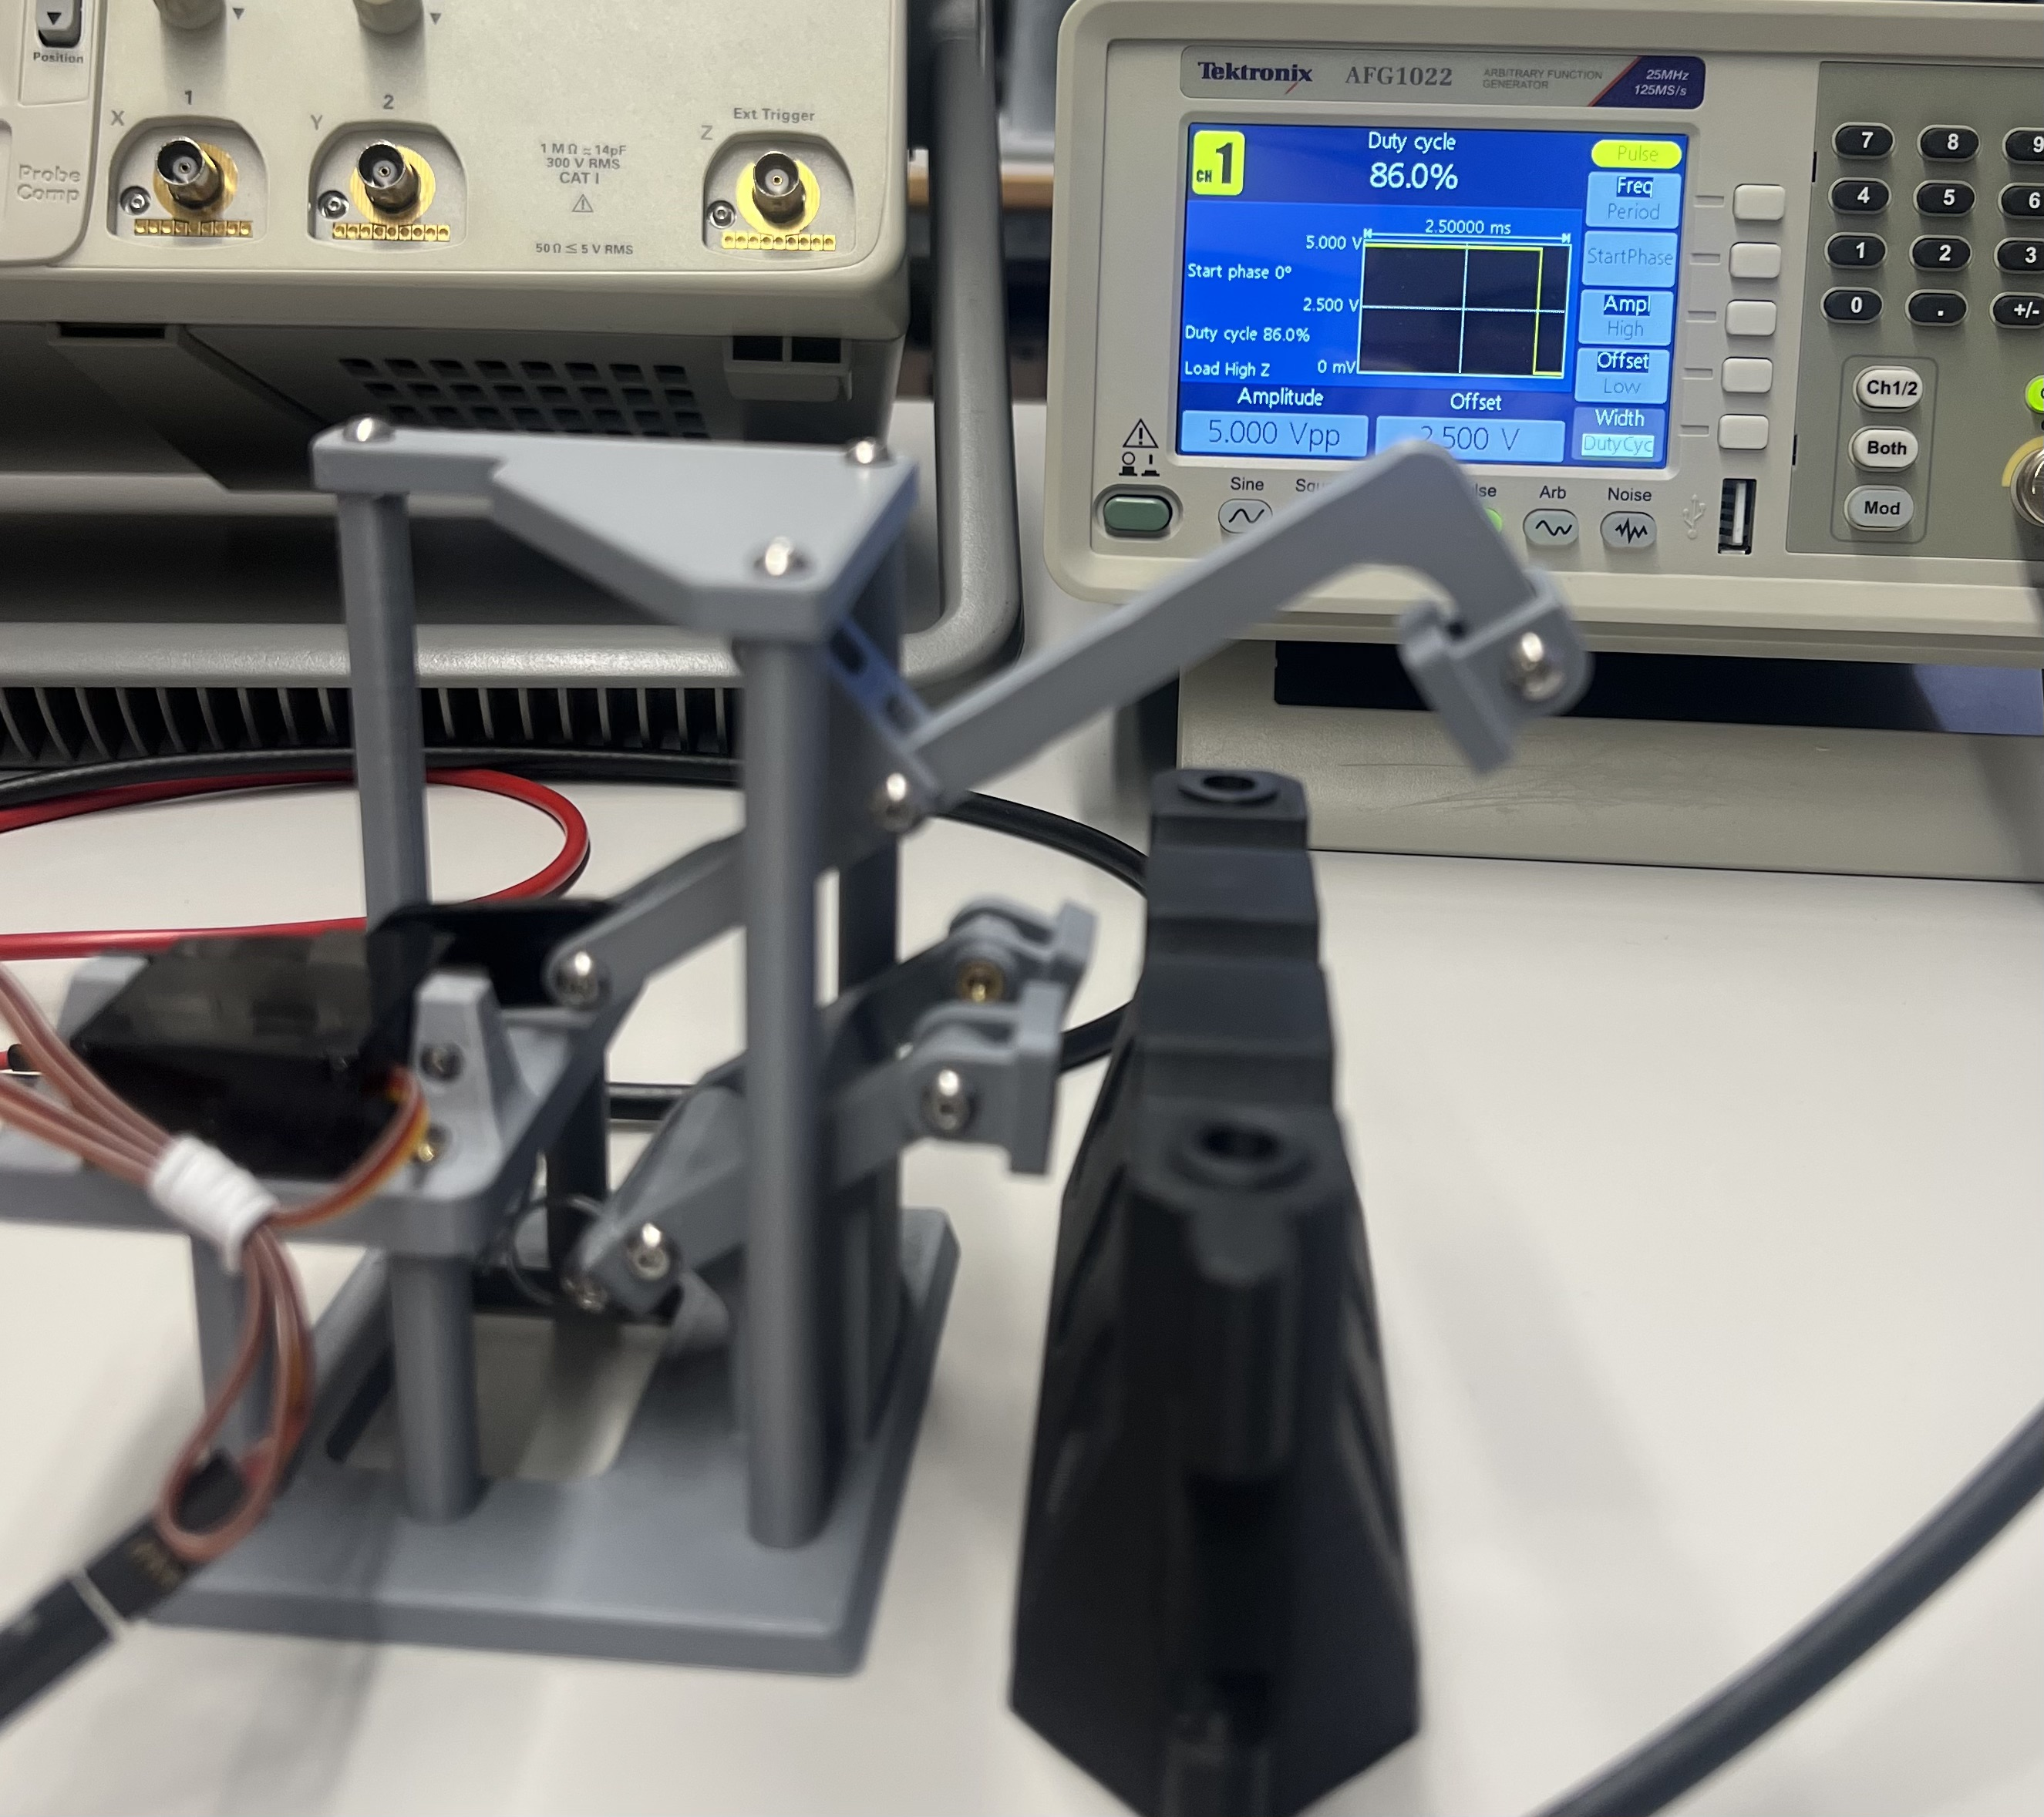
\includegraphics[width=0.8\linewidth]{img/ServoGreifferoffen.jpeg}
    \caption{Greiferposition offen: Duty Cycle 86\%}
    \label{fig: Greiferposition offen: Duty Cycle 86}
\end{figure}

\newpage

Der nächste Messpunkt ist bei dem Zeitpunkt nach dem man den den Duty Cycle so minimiert hat, bis der Greifer das Hindernis klemmt aber noch nicht angehoben hat. Dies sieht man in der unten stehenden Abbildung \ref{fig: Greiferposition eingeklemmt: Duty Cycle 47}.

\begin{figure}[H]
    \centering
    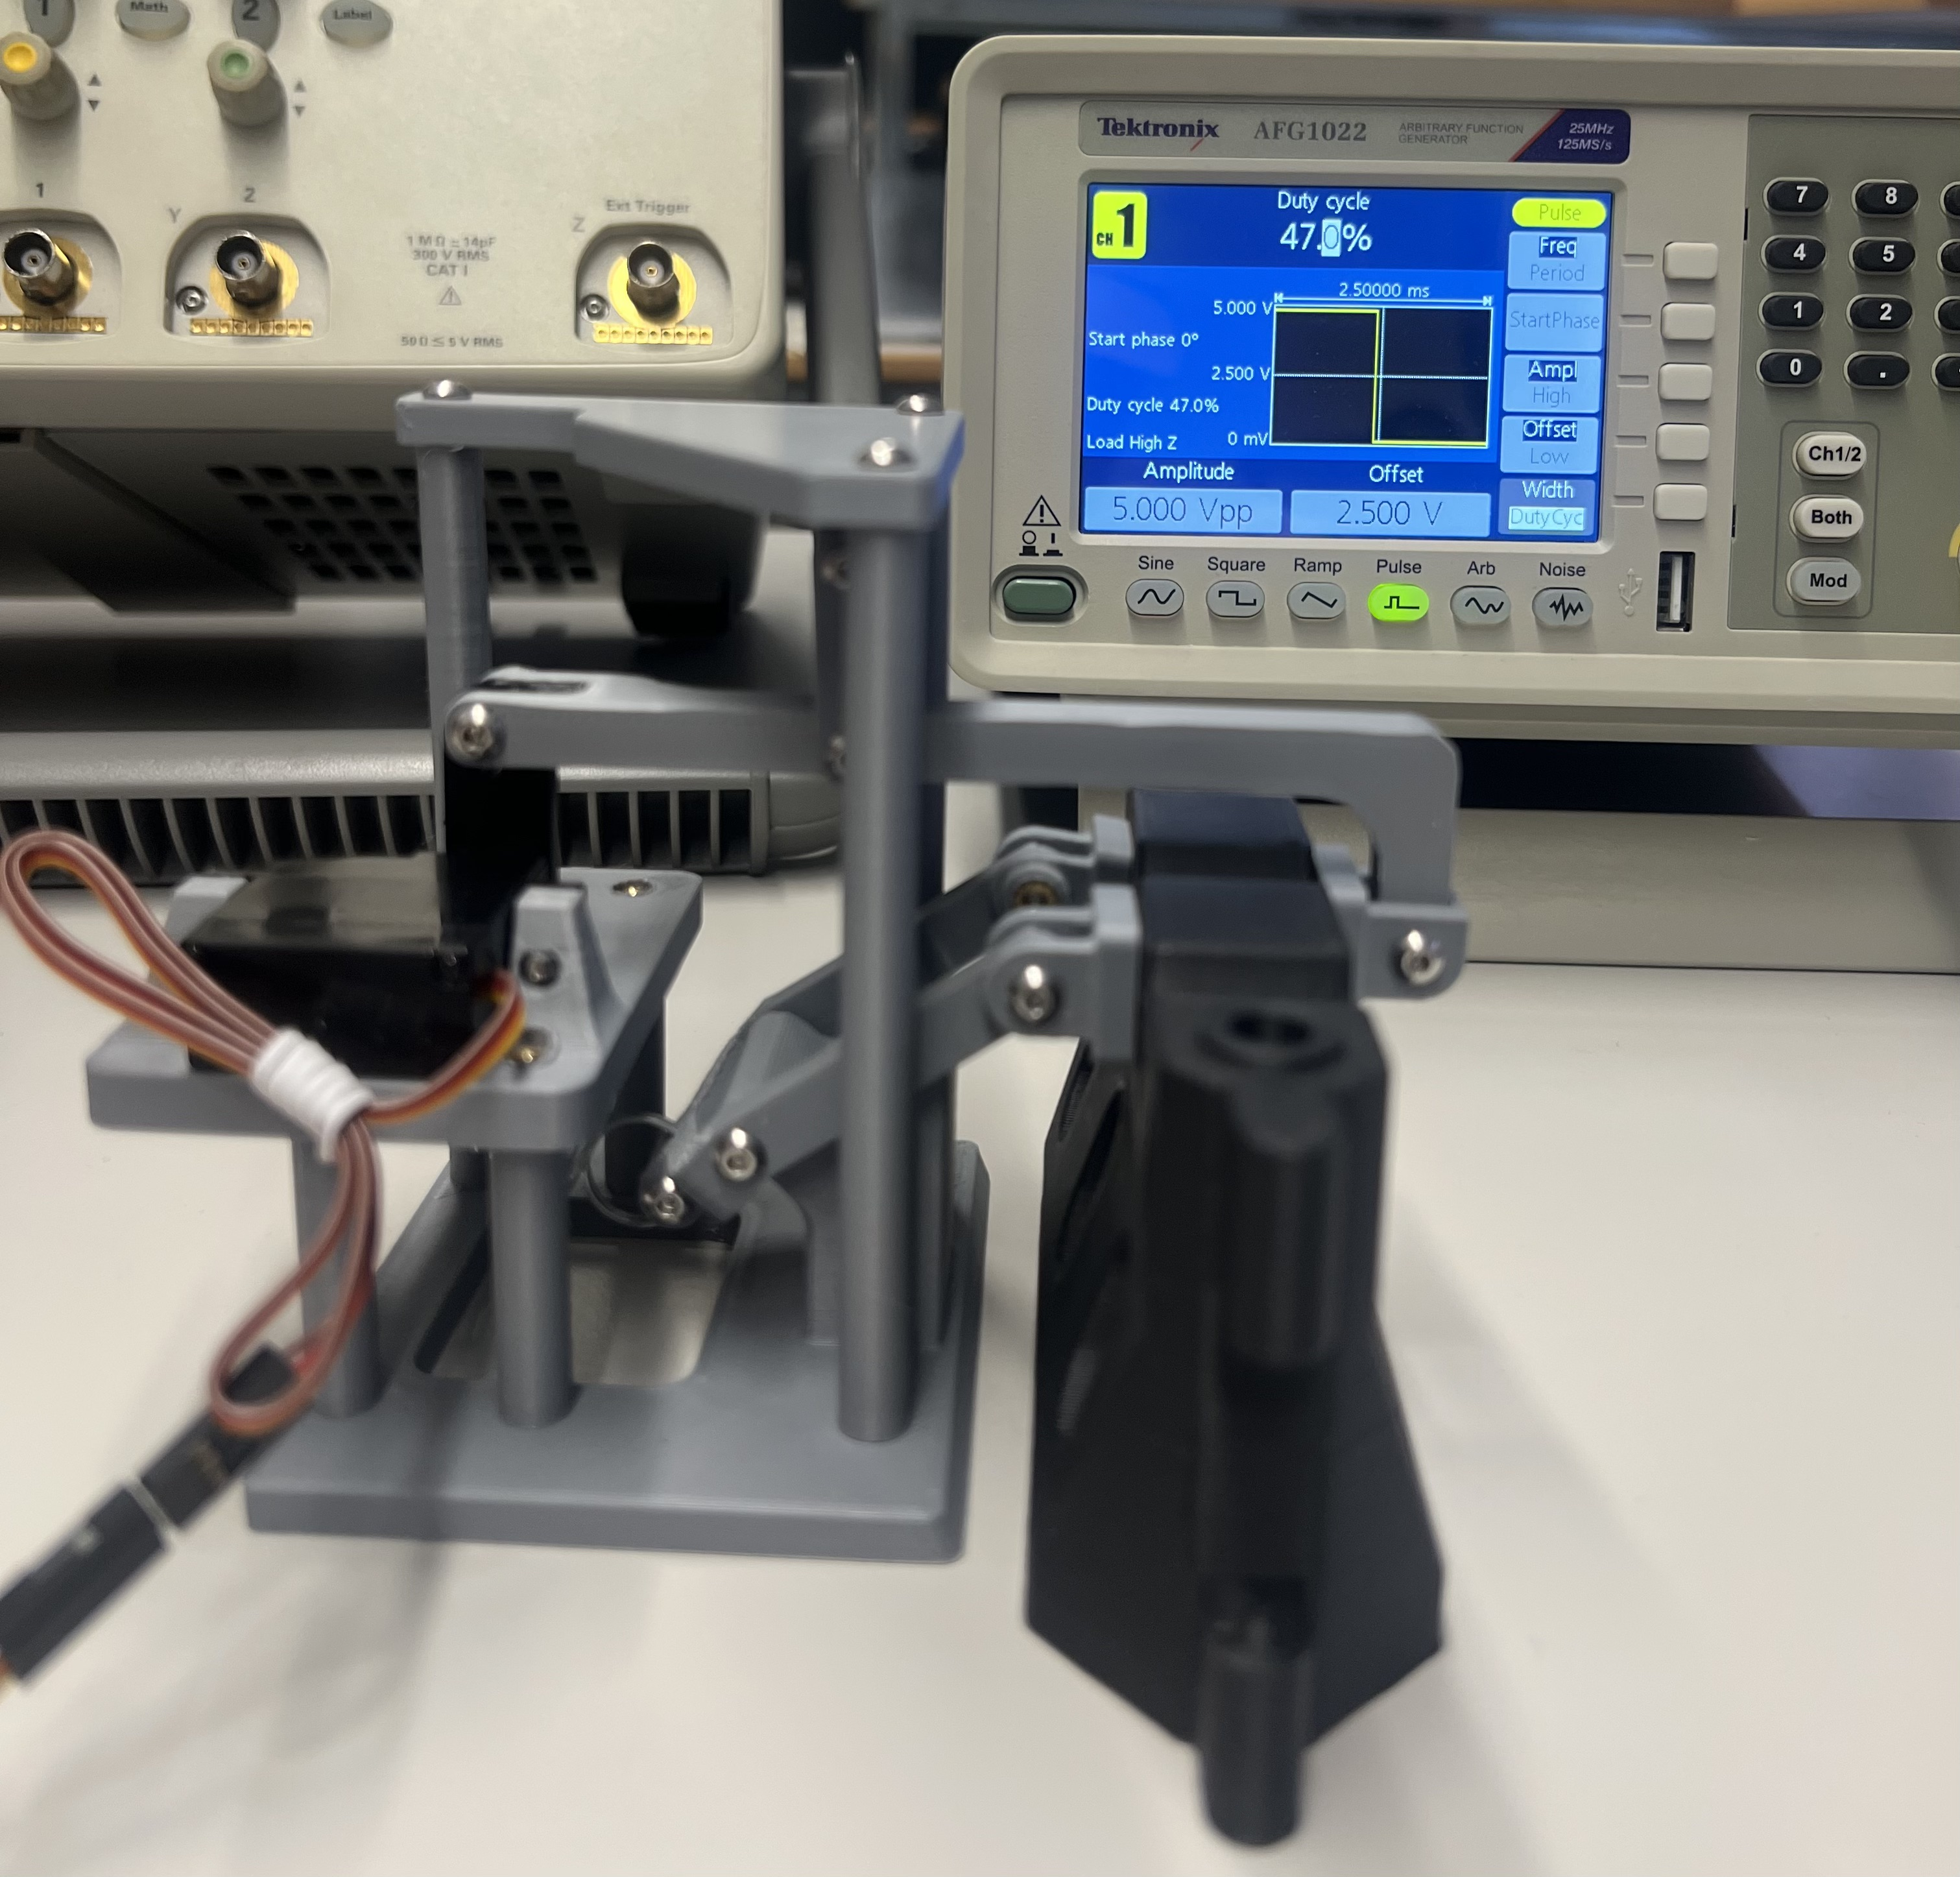
\includegraphics[width=0.8\linewidth]{img/ServoGreiferKlemmt.jpeg}
    \caption{Greiferposition eingeklemmt: Duty Cycle 47\%}
    \label{fig: Greiferposition eingeklemmt: Duty Cycle 47}
\end{figure}

\newpage

Damit man der Anforderung von Tabelle \ref{tab:test-gripper-prototype-1} mit der Hubhöhe gerecht werden kann musste der Duty Cycle auf 32\% reuziert werden. Somit kann man auf der Abbildung \ref{fig: Greiferposition angehoben: Duty Cycle 32} das um 7.5mm angehobene Hindernis erkennen.

\begin{figure}[H]
    \centering
    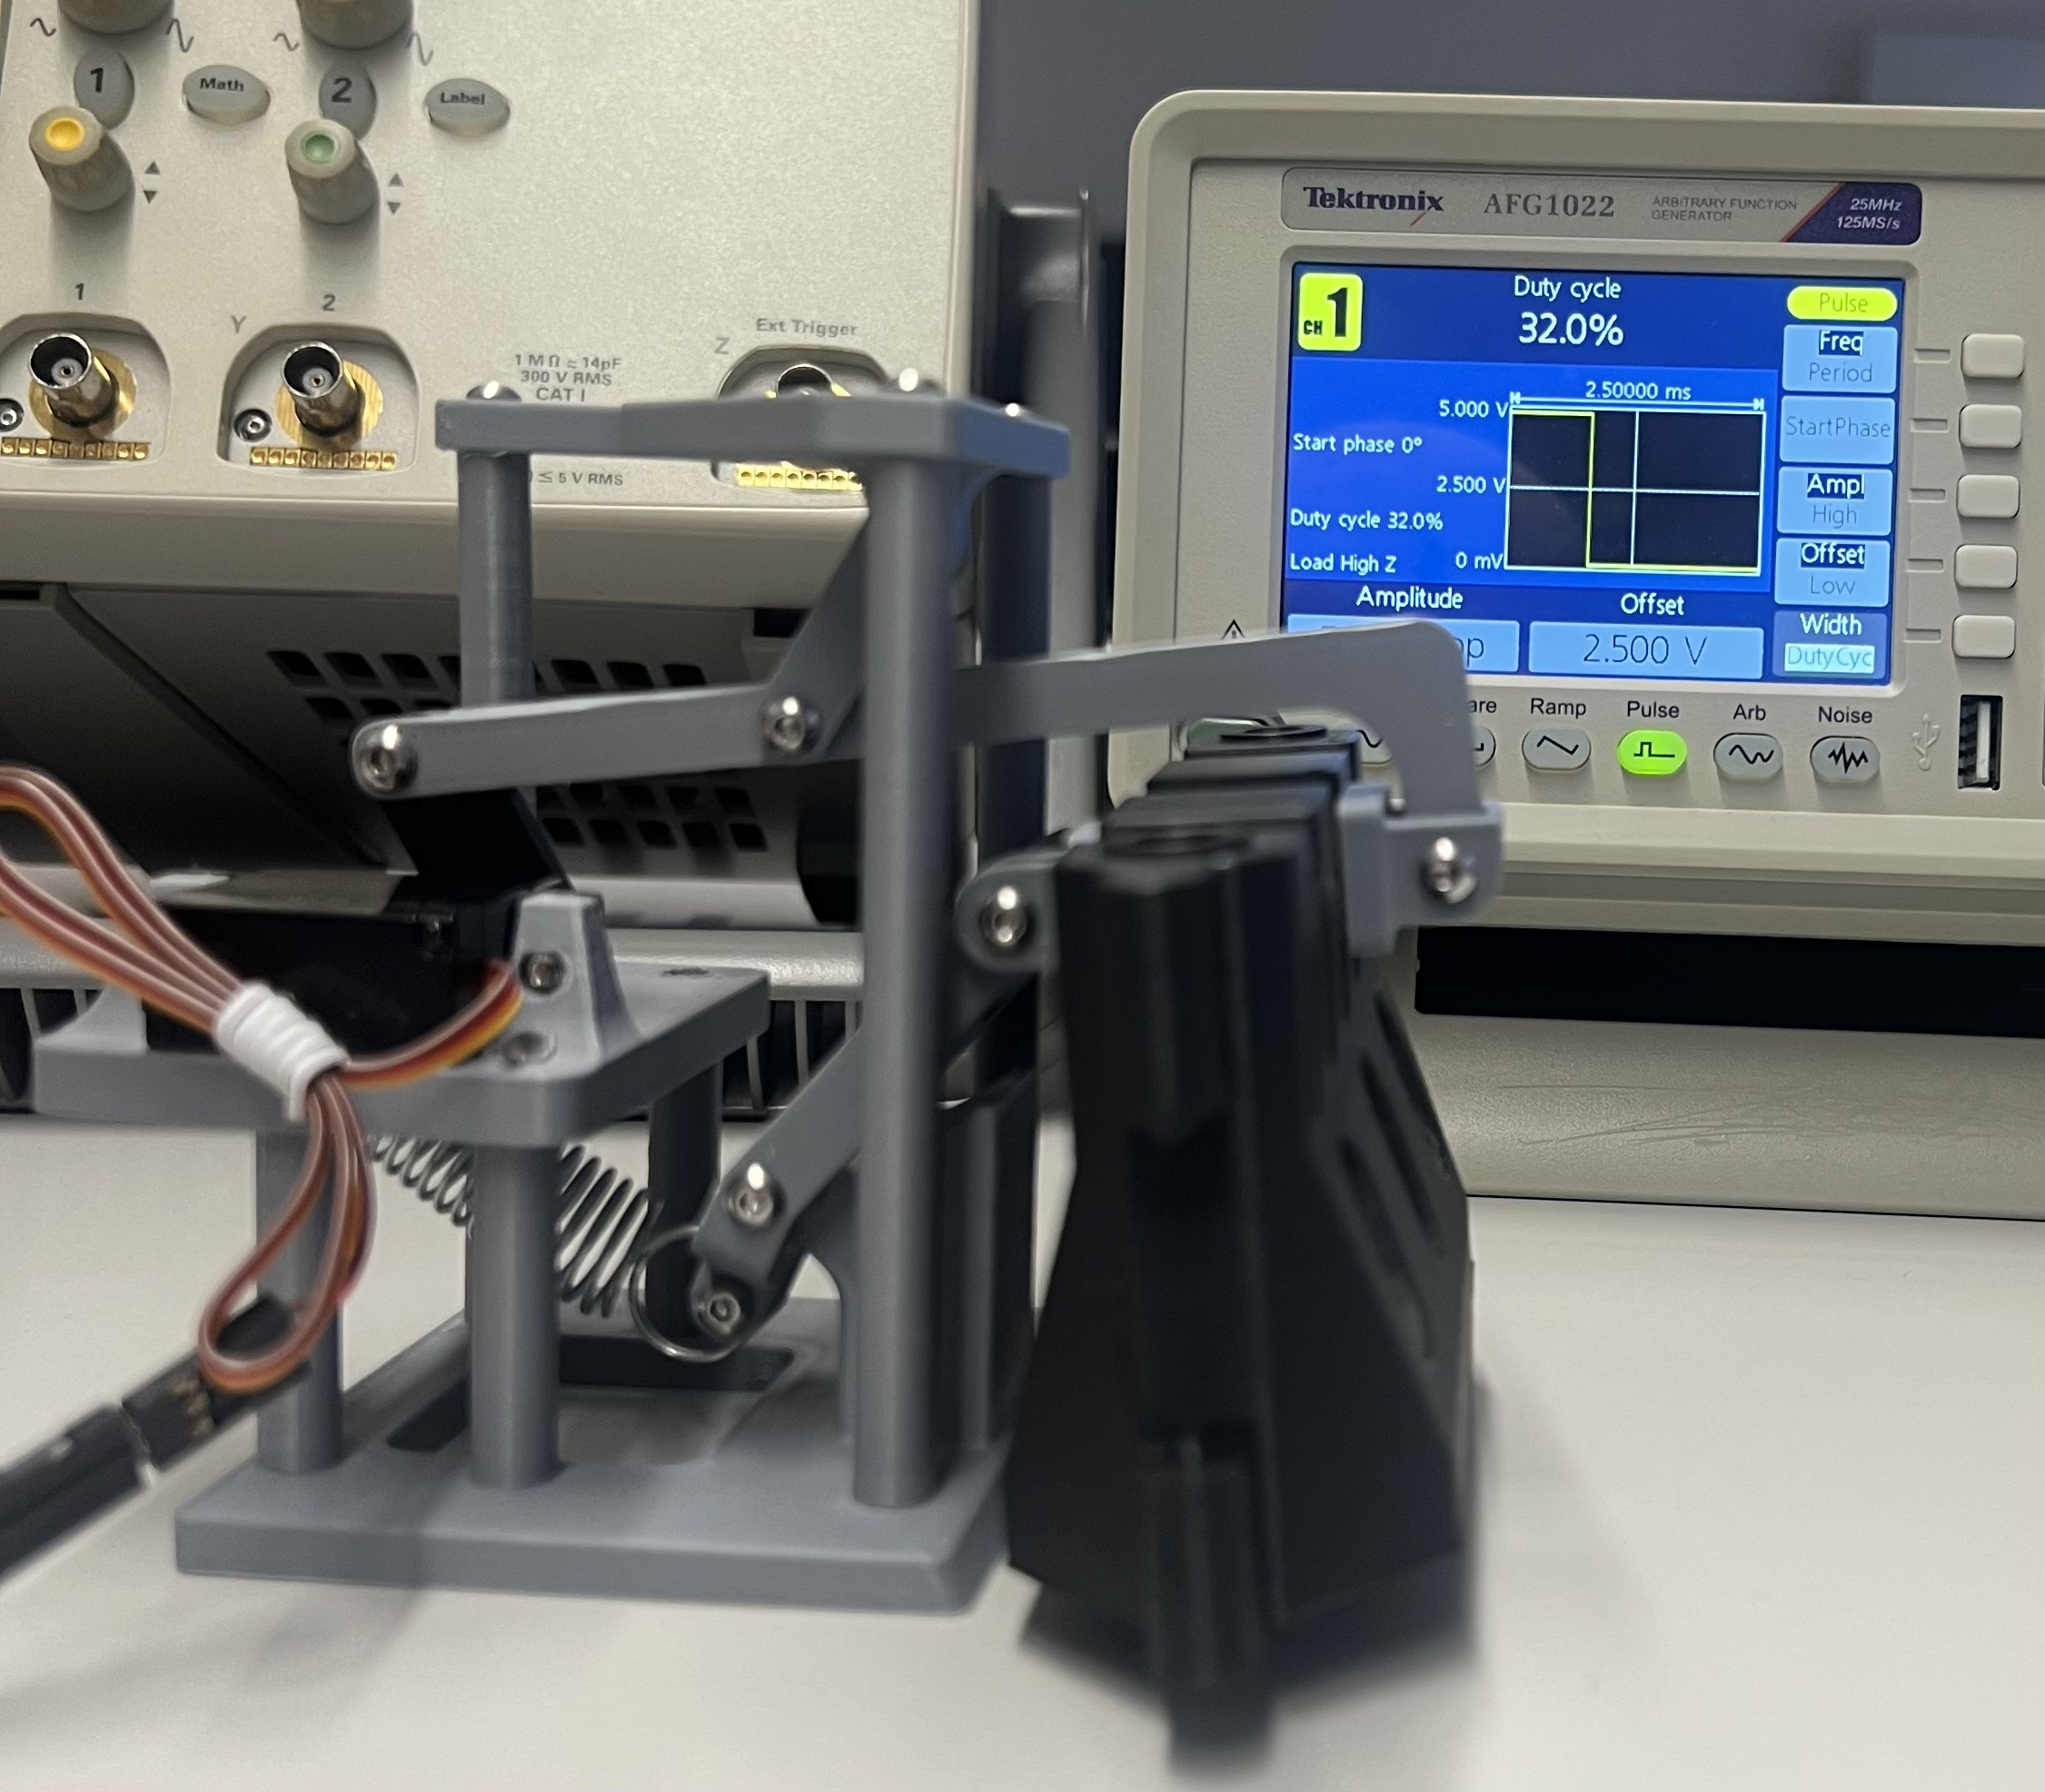
\includegraphics[width=0.8\linewidth]{img/ServoHindernisAngehoben.jpeg}
    \caption{Greiferposition eingeklemmt: Duty Cycle 32\%}
    \label{fig: Greiferposition angehoben: Duty Cycle 32}
\end{figure}